\subsection{Bemeneti és kimeneti paraméterek}
\subsubsection{One Hot kódolás}
A fonéma azonosítására az OneHot kódolást alkalmaztuk (/!TODO referencia), azaz minden fonémára 40 paramétert generáltunk. A már megismert fonéma cimkéket kiegészítettük a fonémában található keretek számával és a keret fonémán belüli elhelyezkedésével, így a kerethez tartozó 215 bemeneti paraméter az alábbiakból tevődik össze:
\subsubsection{Bemeneti paraméterek}
\begin{minipage}{0.5\textwidth}
\begin{itemize}
	\item 0-200 A 40 paraméter a kvinfónra(2-1-2)
	\item 200-213 Fonéma cimkék
	\item 213 A fonémán belüli keretek száma
	\item 214 A keret elhelyezkedése a fonémán belül
\end{itemize} 
\end{minipage} \hfill
\begin{minipage}{0.5\textwidth}
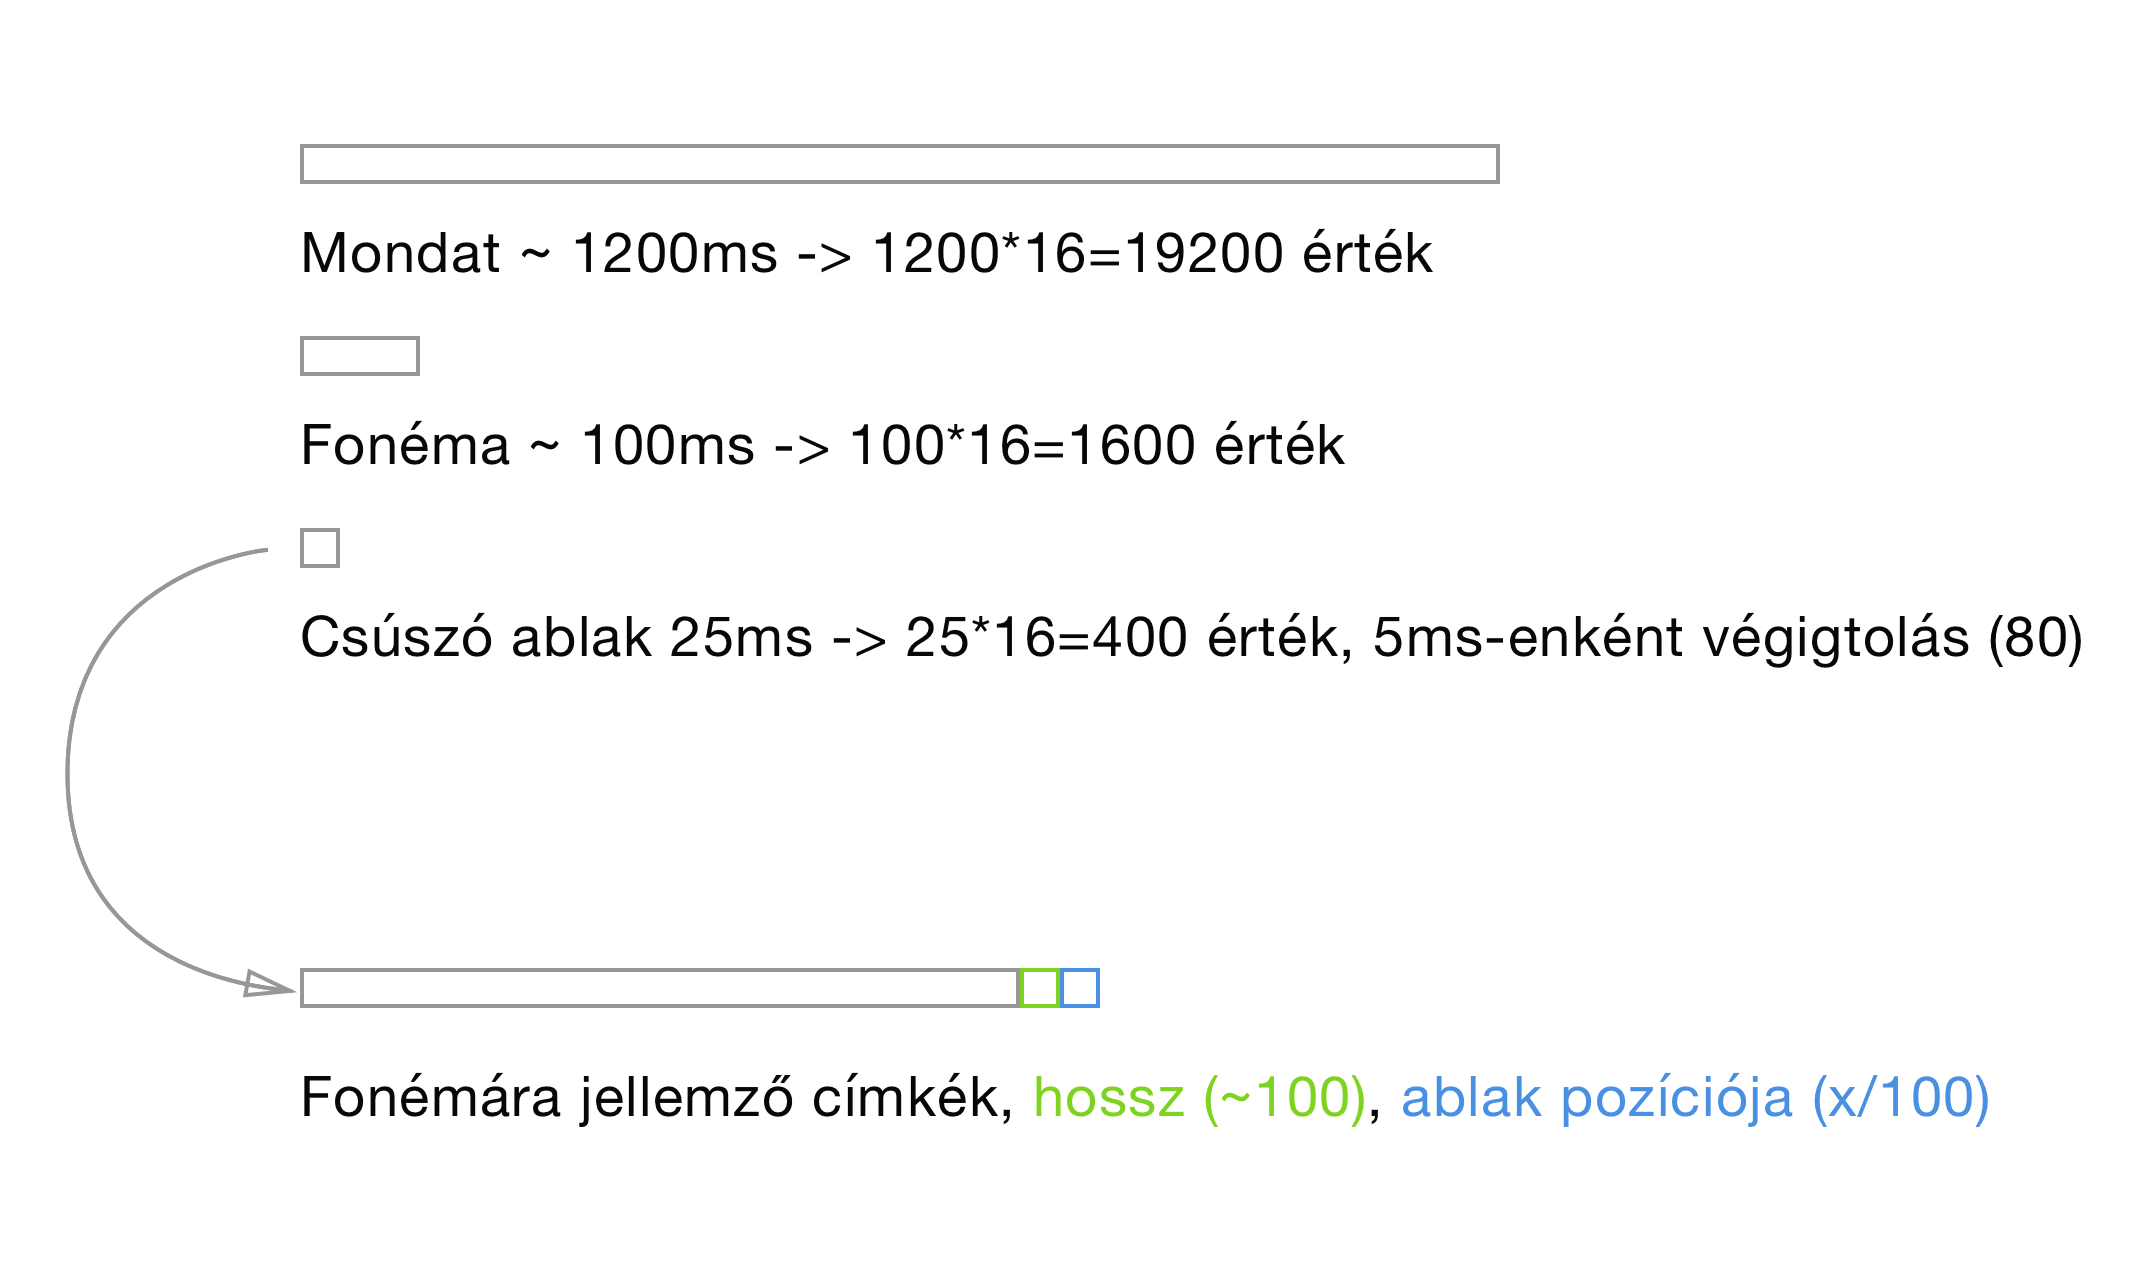
\includegraphics[width=5.5cm,keepaspe5ctratio]{tag_struct}
\end{minipage} \hfill
\subsubsection{Kimeneti paraméterek}
\begin{itemize}
	\item 215 a keret hangmagasság értéke
	\item 216-242 a Mel-Cepstrum 26 paramétere
	\item 242 a fonémán belüli keretek száma
\end{itemize}
\subsection{Spektrális és gerjesztési paraméterek}
Mint említettük a prediktálás alapja a spektrális és gerjesztési paraméterek megadása keretenként. Ezen paraméterek segítségével a PyPSTK (/!TODO ref) python csomag használásával állíthatjuk elő az audio kimenetet, valamint hasonlóképpen ezt a csomagot használjuk az adataink a tiszta hangból való előállítására.
\subsubsection{Mel-Cepstrum}
/!TODO

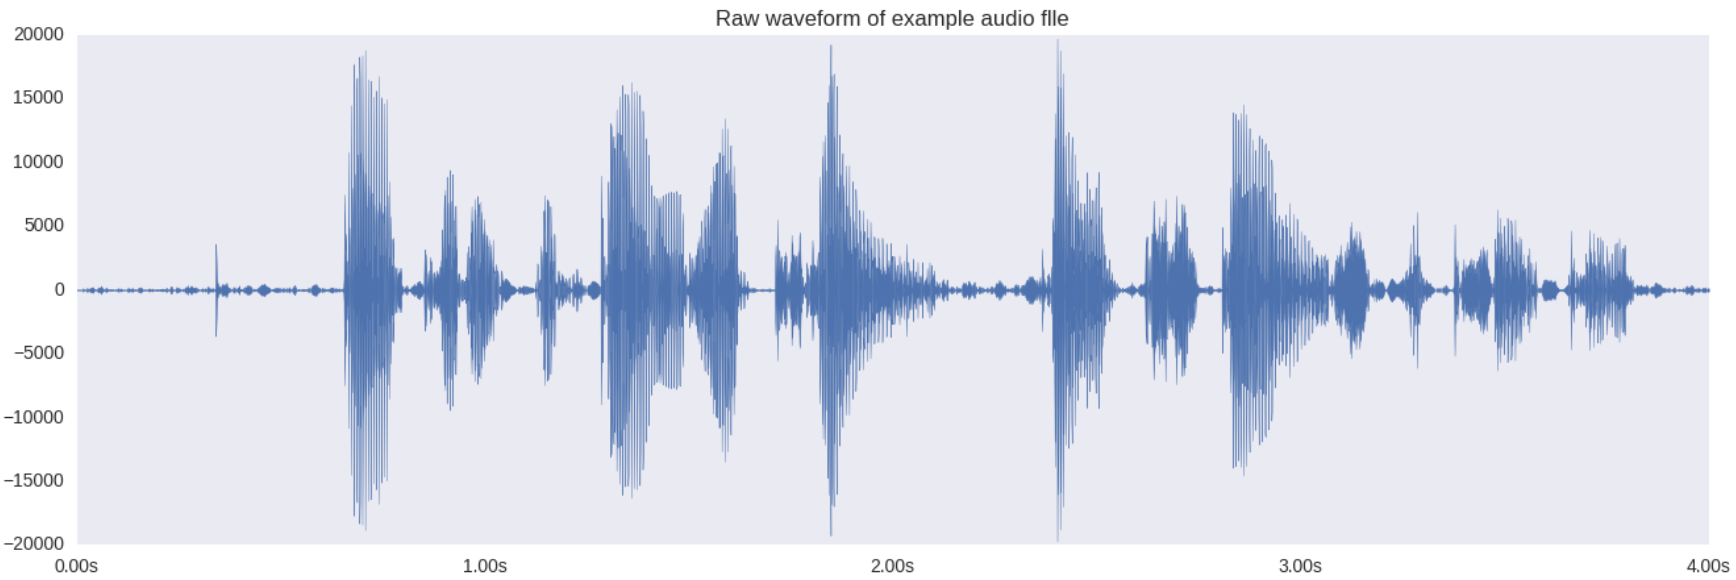
\includegraphics[width=\textwidth,keepaspectratio]{audio_raw}

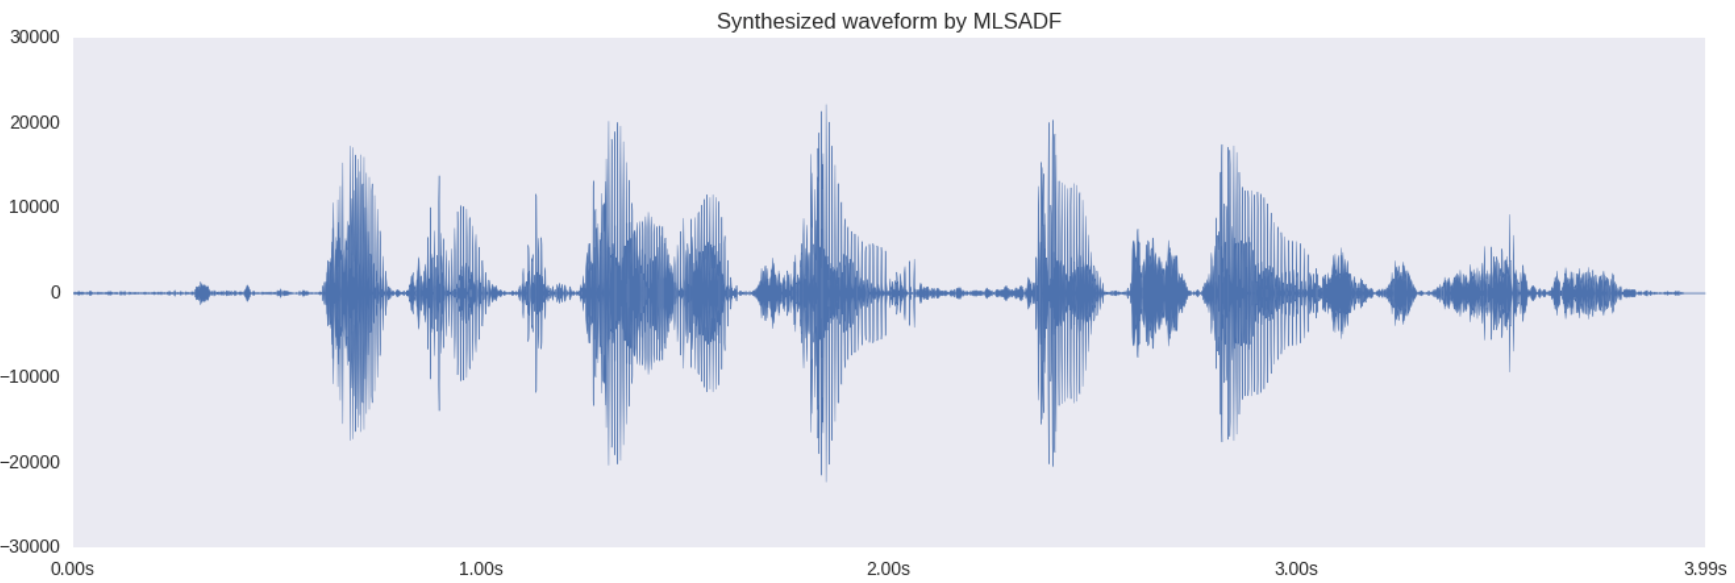
\includegraphics[width=\textwidth,keepaspectratio]{audio_mc}